\documentclass{article}
\usepackage{graphicx,epsfig,amssymb,amstext,amsmath}
\begin{document}
  %-----------------------------------------------------------
  \title{EECS 428 Project}
  \author{Ian Dimayuga}
  \maketitle
  %-----------------------------------------------------------

  \section{Correctness of Simulation}
    \subsection{Exponential Flows}
      \paragraph{}
        The simulation code specifies an average on time of $\mu = 60$ seconds, and an average off time of $w = 180$ seconds.
        The total duration of the simulation $S = 2000$ seconds, and the number of unidirectional browser flows was $n = 30$.
        The total number of bytes transmitted by the exponential flows in one direction was measured to be $T = 111141750$ bytes, or approximately 106 MB.

      \paragraph{}
        Theoretically, the total number of bytes transmitted is given by the equation $T = \dfrac{S n \mu r}{\mu + w}$, where $r$ is the average on-time rate of 56 kbps.

      \paragraph{}
        If we evaluate the equation for $T$, we get $T = 107520000$ bytes, or 103 MB. This matches the measured value of $T$.
        Dividing this by $S$ gives us an average rate of 53760 B/s, or about 0.41 Mbps.

    \subsection{Pareto Flows}
      \paragraph{}
        For the Pareto flows, we specify an average on time $\mu = 500$ milliseconds, and an average off time of $w = 60$ seconds.
        The Pareto on-time rate $r$ was 128 kbps.
        The total number of pareto bytes measured was $T = 8406450$ bytes, or approximately 8 MB.

      \paragraph{}
        If we evaluate the same equation for $T$, we get $T = 8124298$ bytes, or 8 MB. This matches the measured value of $T$.
        Dividing this by $S$ gives us an average rate of 4062 B/s, or about 0.03 Mbps.

    \subsection{Delayed Acknowledgements}
      \paragraph{}
        All DelACK timeouts were measured to be 50ms as specified.
        There are 10905 DelACK timeouts, and 432445 immediate ACKs triggered by data packets.
        The TCP packet to ACK ratio is still 2.

    \subsection{Elephants}
      \paragraph{}
        Given the bandwidth taken up by the Exponential (UDP) flows, TCP packets are left with $10 - r_{exp} = 9.5$ Mbps of bandwidth through the central link.
        This can be corroborated by measuring the amount of data being ACKed over time.
        As shown in Figure \ref{fig:ack_plot}, the data ACKed over time does not change as the first Elephant finishes at 704s.
        The initial slope of this graph (9.5 Mbps) shows that the link is at full utilization all the way until the second Elephant finishes.
        There are distinct slope changes when the second and third Elephants finish.
        Furthermore, the total number of bytes ACKed at the conclusion of the trace is 1.21 GB, which is equal to the sum of the three 400 MB files and the 16 MB of total data in the pareto flows.

    \begin{figure}[h]
      \begin{centering}
        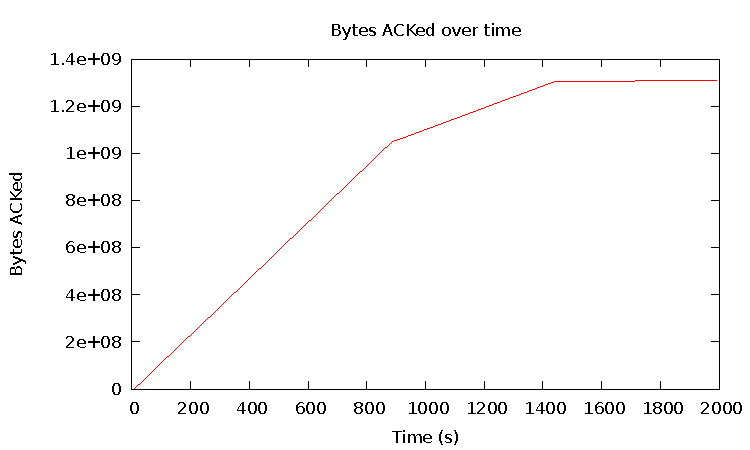
\includegraphics{ack_plot}
        \caption{The cumulative number of bytes ACKed at the source, taken every 10 seconds.}
        \label{fig:ack_plot}
      \end{centering}
    \end{figure}

  \section{Elephant Utilization}

    \paragraph{}
      As shown in figure \ref{fig:elephant_bw}, the total Elephant flow bandwidth usage stays at around 9 Mbps until the second elephant finishes at 885s.
      However, it does not remain at full utilization after this time.
      This is also indicated by the change in slope in \ref{fig:ack_plot}.

    \begin{figure}[h]
      \begin{center}
        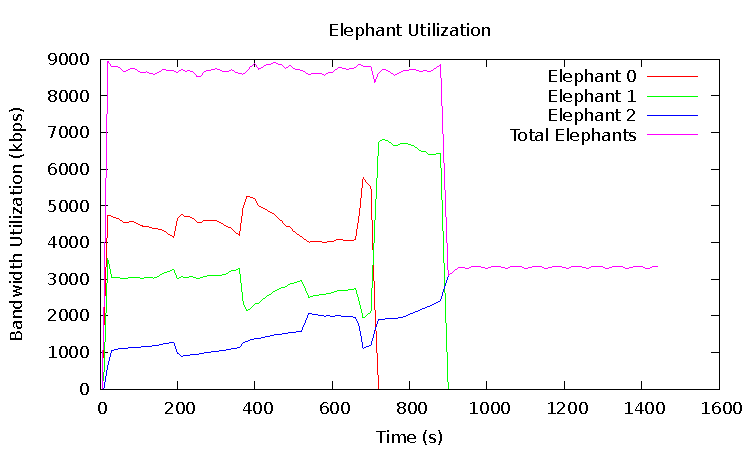
\includegraphics{elephant_bw}
        \caption{The bandwidth utilization of each elephant, as well as the total bandwidth utilization of all elephants.}
        \label{fig:elephant_bw}
      \end{center}
    \end{figure}

    \subsection{}


\end{document}
